% пользовательская сессия
\begin{frame}
  \frametitle{Пользовательская сессия}

  \begin{center}
    \begin{block}<1->{Многопользовательская система?}
      Надо представиться системе. Логин и пароль.
    \end{block}

    \begin{block}<2->{Как может выглядеть}
      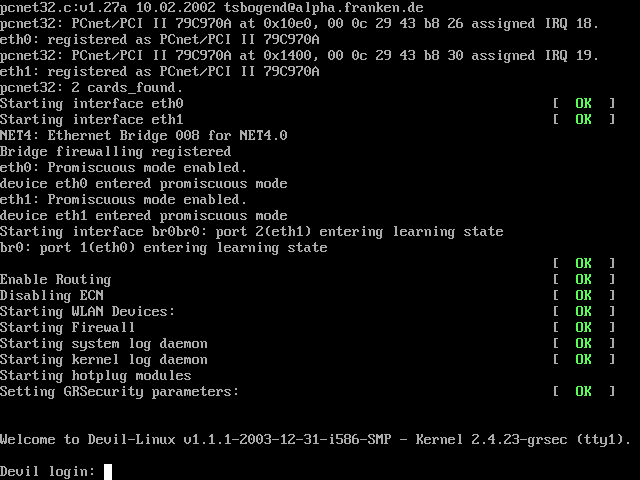
\includegraphics[height=2.5cm]{console-login-screenshot}
      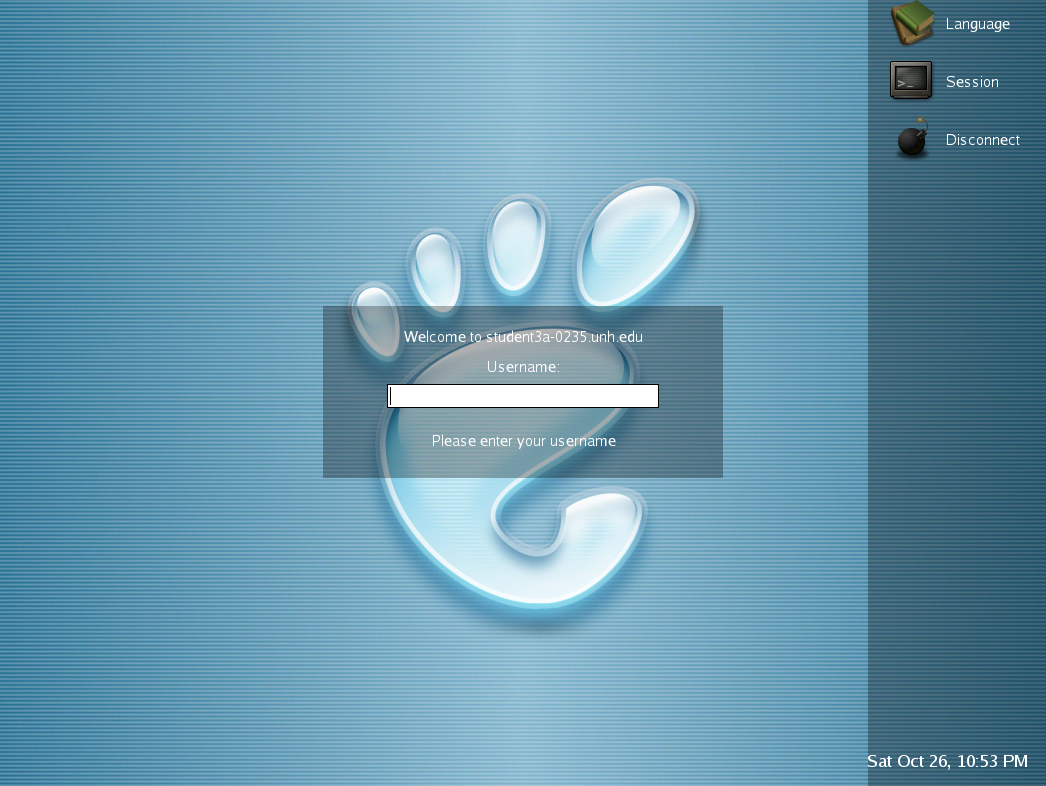
\includegraphics[height=2.5cm]{gdm-login-screenshot}
      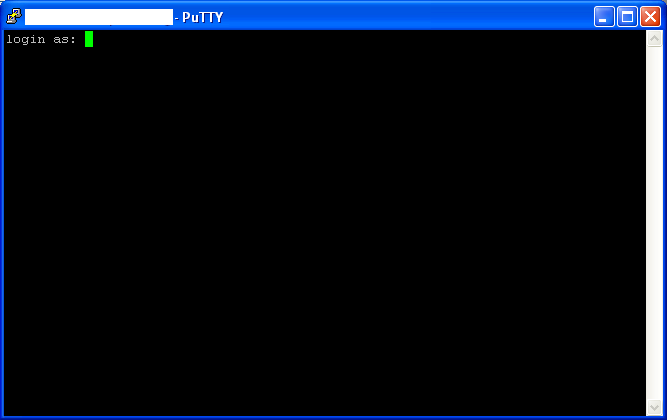
\includegraphics[height=2.5cm]{putty-login-screenshot}
    \end{block}

    \begin{block}<3->{Виды сессий}
      \begin{itemize}
        \item локальные и удалённые (сетевые)
        \item текстовые и графические
      \end{itemize}
    \end{block}

  \end{center}

\end{frame}

\begin{frame}
  \frametitle{Входим удалённо. SSH}

  \begin{center}

    SSH - \emph{S}ecure \emph{SH}ell
    \newline \pause

    Протокол удалённой работы по сети для Linux.

    Много реализаций клиентов и серверов.
    \newline
    \pause

    \emph{Как может выглядеть:}
    \newline
    \fbox{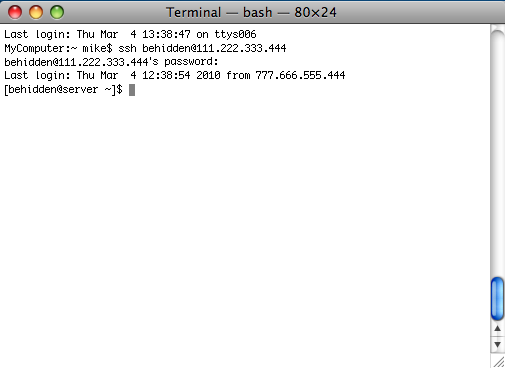
\includegraphics[height=3.5cm]{console-ssh-screenshot}}
    \emph{ }
    \fbox{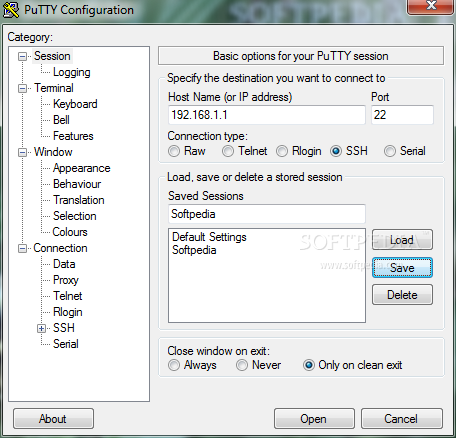
\includegraphics[height=3.5cm]{putty-config-screenshot}}
  \end{center}

\end{frame}

\begin{frame}
  \frametitle{Выход из матрицы}

  \begin{center}
    
\includegraphics[height=5.5cm]{matrix-screenshot}
    \pause
    \newline
    \begin{itemize}
      \item Команда \emph{exit}
      \item Команда shell \emph{logout}
      \item Hotkey \emph{Ctrl+d}
      \item Закрыть клиента
    \end{itemize}
  \end{center}

\end{frame}
